\documentclass[11pt]{article}

\usepackage[review]{acl}
\setlength{\linenumbersep}{6pt}
\AtBeginDocument{\switchlinenumbers*}
\makeatletter
% TeX Live 2026 lineno can place first-page ACL review numbers in the column
% gutter because of the \twocolumn[\maketitle] title block. Keep the review
% ruler on body pages, but suppress the visually broken first-page numbers.
\let\acl@orig@makeLineNumberLeft\makeLineNumberLeft
\let\acl@orig@makeLineNumberRight\makeLineNumberRight
\renewcommand\makeLineNumberLeft{\ifnum\value{page}=1\relax\else\acl@orig@makeLineNumberLeft\fi}
\renewcommand\makeLineNumberRight{\ifnum\value{page}=1\relax\else\acl@orig@makeLineNumberRight\fi}
\makeatother

\usepackage{times}
\usepackage{latexsym}
\usepackage[T1]{fontenc}
\usepackage[utf8]{inputenc}
\usepackage{microtype}
\usepackage{inconsolata}
\usepackage{graphicx}
\usepackage{booktabs}
\usepackage{multirow}
\usepackage{tabularx}
\usepackage{enumitem}
\usepackage{amsmath}
\usepackage{amssymb}

\newcommand{\task}{evidence-grounded response resolution}
\newcommand{\dataset}{RegTrace-SEC}
\newcommand{\cmsdataset}{RegTrace-CMS}
\newcommand{\framework}{RegTrace-Agent}

\title{\framework{}: Learning Regulatory Review Policies from\\
Context-to-Feedback Traces}

\author{Anonymous ACL submission}

\begin{document}
\maketitle
\begin{abstract}
Many regulatory and compliance workflows are not ordinary document QA: they ask whether an organization has actually closed a requested fix in later evidence. The hard part is both modeling and data orchestration, because each domain exposes different pieces of the trace: a request, a response, revised evidence, review labels, written feedback, and sometimes later reviewer behavior. We introduce \framework{}, a trace-to-feedback framework that constructs these roles from heterogeneous regulatory corpora, trains a runtime reviewer under a strict evidence boundary, and recycles adjudicated failures as feedback for the next reviewer policy. Our primary instantiation, \dataset{}, is a 472-example public EDGAR benchmark of SEC comment-letter review with amended-filing evidence, structured feedback, and later same-topic SEC follow-up; we further adapt the same framework to CMS corrective plans and FDA warning-to-closeout traces. Under fixed test-time evidence, full natural-language feedback is the strongest reviewer-training signal, outperforming handwritten prompting, MIPROv2, scalar/category GEPA variants, lexical and encoder scorers, and typed decision gates. Evidence ablations, a stratified human-reviewed audit, external SEC follow-up, and CMS/FDA studies support context-to-feedback traces as a portable supervision format for evidence-grounded regulatory review.
\end{abstract}

\section{Introduction}

Financial NLP is increasingly evaluated on long documents, retrieval, and domain-specific reasoning. BloombergGPT, FinGPT, FinBen, FinanceBench, FinQA, TAT-QA, and ConvFinQA show the promise of financial LLMs and the difficulty of grounding answers in financial evidence \citep{wu2023bloomberggpt,yang2023fingpt,xie2024finben,islam2023financebench,chen2021finqa,zhu2021tatqa,chen2022convfinqa}. Recent FinNLP work similarly studies retrieval-augmented financial QA, SEC filing QA, factuality judging, finance benchmarks, and evasive-answer detection \citep{lithgow2025rag,lai2025secqa,klimaszewski2025avenibench,wu2025nli,nuaimi2025evasive}. Yet many high-value compliance workflows are not static QA tasks. They are repair-review loops: a reviewer requests a fix, an organization claims it has acted, and the next reviewer must decide whether the visible artifact actually closes the obligation.

In such workflows, a regulator, auditor, lender, or control function requests a correction, explanation, disclosure, or supporting artifact. The organization may respond that it has revised a filing, submitted a plan, filed an exhibit, changed a policy, or completed remediation elsewhere. A reviewer must then decide whether visible revised evidence satisfies the original request. This is harder than judging whether the response sounds cooperative: a company may say it revised a forecast disclosure, while the amended filing still omits requested entity-level assumptions; a nursing facility may submit a corrective plan that includes staff education, while leaving one cited resident-safety failure unaddressed. We call this problem \task{}.

The task has a distinctive data structure. Each example may contain a prior request, a response that only claims a fix, revised or corrective evidence that must be inspected, feedback about what remains missing, and later reviewer behavior. This is related to fact verification and document-level legal NLI \citep{thorne2018fever,koreeda2021contractnli}, but the central question is whether a documented obligation has been materially closed by a later artifact.

The central data challenge is adaptive schema orchestration. Different regulatory corpora expose different parts of the review trace. SEC comment-letter correspondence exposes staff requests, company responses, amended filings, and sometimes later same-topic follow-up. CMS nursing-home inspection data exposes deficiency narratives and Plans of Correction, but the adequacy rubric changes from disclosure closure to corrective-action sufficiency. FDA warning-letter data often lacks public company response letters, so a useful framework should reshape the task into warning-to-closeout trace verification rather than forcing a missing response role. A reusable system therefore needs more than a classifier. It needs a constructor that decides which trace roles exist, which fields are visible at runtime, which fields are audit-only feedback, and whether the domain supports response-adequacy review or requires a related trace task.

Our primary public benchmark comes from U.S. Securities and Exchange Commission (SEC) comment-letter review, because it exposes the richest trace. SEC staff issue comments asking companies to expand disclosure, clarify accounting treatment, remove unsupported statements, or file additional materials. Companies respond in writing, often saying that disclosure has been ``revised accordingly.'' After review completion, the SEC releases staff letters and company responses through EDGAR, and later same-topic SEC follow-up comments sometimes reveal that a requested fix still did not land. Accounting research treats comment letters as economically meaningful regulatory events \citep{cassell2013sec,bozanic2017sec,baugh2023auditor,ryans2021comment}; for NLP, they provide public traces of request, response, evidence, feedback, and external reviewer behavior.

The practical stakes are material. The SEC describes the review process as a mechanism for monitoring and improving compliance with disclosure and accounting requirements, where companies generally respond to each staff comment and may amend filings \citep{sec2026edgarcorrespondence}. A recent practitioner review reports that, from review years 2021--2025, SEC reviews took about 54 days on average, increased to 69 days in 2025, and involved roughly 1.4 comment letters per review on average \citep{deloitte2026commentletters}. Academic evidence further links accounting-related comments to higher remediation costs, in part because they take more time to resolve \citep{cassell2013sec}. Even without observing firms' internal legal, accounting, and audit bills, the workflow is plainly costly: unresolved issues can trigger additional correspondence, amended filings, delayed closure, and repeated expert review.

We introduce \framework{}, a framework that turns heterogeneous review corpora into context-to-feedback review systems. A domain \textsc{TraceSpec} constructor maps local documents into request, response, evidence, label, feedback, corroboration, and hidden-field roles. An evidence module retrieves revised artifacts. A runtime reviewer decomposes obligations, verifies claims against visible evidence, and emits a guarded verdict. Offline adjudication converts failures into scalar, category, or natural-language feedback, which is used to improve the next reviewer policy. The empirical question is not whether hidden adjudication notes can be placed into a test prompt. They cannot. The question is whether written feedback from prior review traces can train a better reusable reviewer under the same runtime evidence boundary. The claim is that feedback-rich review traces are a portable supervision format for evidence-grounded regulatory review.

We make four contributions. First, we define \task{} and introduce \framework{}, a trace-to-feedback framework with adaptive construction, retrieval, review, adjudication, optimization, and guarded reuse modules. Second, we release \dataset{}, a 472-example public EDGAR benchmark with SEC comments, company responses, amended-filing snippets, visible-evidence labels, structured feedback, split files, model outputs, audit metadata, and follow-up corroboration. Third, under fixed test-time evidence, we show that full natural-language feedback is the strongest reviewer-training signal across grouped, temporal, and topic-holdout SEC evaluations. Fourth, we validate and stress-test the framework with evidence ablations, feedback ablations, prompt-evolution analysis, a stratified human-reviewed audit, later-SEC-follow-up corroboration, CMS corrective-plan adaptation, and an FDA warning-to-closeout stress test.

\section{Related Work}

\paragraph{Financial NLP and evidence grounding.}
FinQA, TAT-QA, ConvFinQA, and FinanceBench evaluate financial reasoning and open-book QA over reports, tables, conversations, and company documents \citep{chen2021finqa,zhu2021tatqa,chen2022convfinqa,islam2023financebench}. Recent FinNLP work emphasizes RAG over financial documents, accessible finance-intelligence benchmarks, factuality and causality judging, SEC filing QA, and evasive-answer detection \citep{lithgow2025rag,klimaszewski2025avenibench,lai2025secqa,nuaimi2025evasive,wu2025nli}. Our task differs by asking whether retrieved revised evidence satisfies a prior regulator request.

\paragraph{Regulatory traces and language feedback.}
Accounting research studies SEC comment letters as regulatory signals, including remediation costs, disclosure effects, recurring disclosure deficiencies, and textual classification of comment-letter topics \citep{cassell2013sec,bozanic2017sec,baugh2023auditor,ryans2021comment}. We instead treat the correspondence as document-grounded supervision for LLM systems. Prompt-programming work treats LLM pipelines as declarative programs whose prompts and demonstrations can be optimized \citep{khattab2023dspy}. MIPROv2 and related optimizers primarily use scalar feedback, while GEPA uses natural-language reflection over execution traces \citep{agrawal2026gepa}. This distinction is central because SEC response errors are naturally textual: missing disclosures, unsupported revision claims, absent exhibits, incomplete analysis, or over-demand beyond the SEC request.

\section{\framework{} Framework}

\framework{} applies when a response claims to satisfy a prior review request by modifying or supplying evidence outside the response itself. Each trace contains a request $q$, response $r$, artifacts $\mathcal{D}$, and optional later reviewer feedback $u^+$. The system retrieves evidence $e=R(q,r,\mathcal{D})$, extracts obligations $o_{1:m}=O(q)$, and applies a verifier $V(q,r,e,o_{1:m})$ whose output is \texttt{resolved} or \texttt{unresolved}. The same trace can produce three feedback channels for learning: scalar correctness, coarse category feedback, and full natural-language feedback describing the request, response action, evidence coverage, and unmet requirement.

\begin{figure*}[t]
\centering
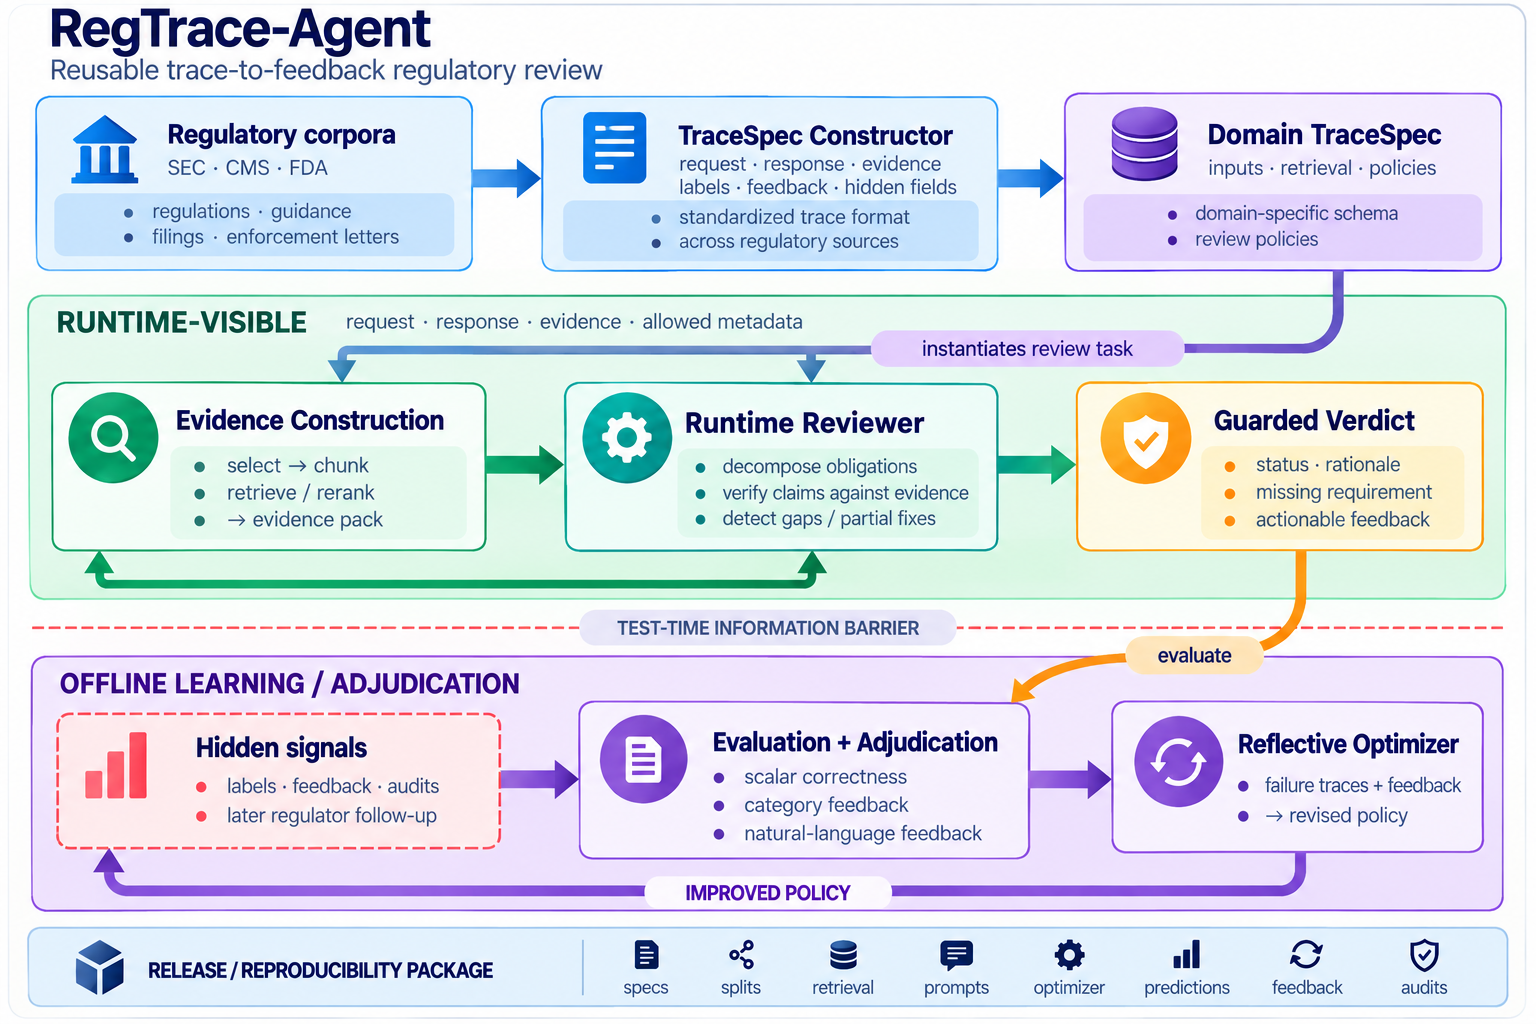
\includegraphics[width=0.95\textwidth]{figures/regtrace_agent_framework_user.png}
\caption{\framework{} architecture. A \textsc{TraceSpec} constructor maps each regulatory corpus into request, response, evidence, label, feedback, and hidden-field roles. The runtime reviewer sees only approved inputs and evidence, performs obligation-level review, and emits a guarded verdict. Offline adjudication, audit, and follow-up signals become scalar, category, and written feedback for policy improvement.}
\label{fig:pipeline}
\end{figure*}

\paragraph{Adaptive construction.}
For a candidate domain $d$, the constructor emits a \textsc{TraceSpec} $S_d=(\phi_d,y_d,f_d,a_d,\rho_d)$, where $\phi_d$ maps local fields into request, response, evidence, metadata, and external-corroboration roles; $y_d$ defines the review label; $f_d$ defines feedback channels; $a_d$ lists fields forbidden at test time; and $\rho_d$ scores utility. If a core role is weak, the constructor reshapes the task rather than forcing the SEC schema. Thus SEC uses staff comment, company response, amended-filing snippets, visible-evidence label, and later same-topic follow-up; CMS-2567 becomes plan-of-correction adequacy review; and FDA warning letters are reshaped into warning-to-closeout trace verification because public company response letters are mostly absent.

\paragraph{SEC instantiation.}
Each SEC example exposes three test-time fields: \texttt{sec\_comment}, \texttt{company\_response}, and raw \texttt{retrieved\_snippets} from amended filings. \texttt{resolved} means visible evidence covers the material request; \texttt{unresolved} means a named item, quantification, exhibit, document, legal analysis, accounting analysis, or other material requirement remains missing. The label is a visible-evidence judgment, not a legal determination or an inference from absence of later follow-up.

We harvest \texttt{UPLOAD} and \texttt{CORRESP} materials from EDGAR, group comments and responses into review threads, and select cases where the company claims a disclosure was added, revised, removed, or filed elsewhere. We identify amended filing candidates using filing metadata, target forms, amendment references, page cues, response dates, and response text. The released prototype searches nearby company filings, excludes \texttt{UPLOAD}/\texttt{CORRESP}, keeps at most eight candidate filings, chunks filing text into 1,800-character windows with 250-character overlap, ranks chunks by salient terms, and passes the top three snippets to an LLM reranker/adjudicator.

\dataset{} contains 472 examples from 109 SEC review threads and 95 companies. It focuses on difficult revision-claim cases: 153 examples are \texttt{resolved}, and 319 are \texttt{unresolved}. The corpus covers seven issue categories, including disclosure issues, risk factors, SPAC disclosure, revenue recognition, crypto, non-GAAP, and cybersecurity. We use grouped, temporal, and topic-holdout regimes. The grouped split holds out entire review threads (229/104/139 train/dev/test). The temporal split trains on 2022--2023 and tests on 2024--2025 (264/64/144). The topic split tests transfer to held-out issue categories (279/68/125), including crypto and non-GAAP cases absent from training categories.

\paragraph{Validation and release.}
Because the benchmark label is a visible-evidence judgment, label validity is part of the contribution. We use three checks: an independent LLM auditor that sees only test-time fields; later same-topic SEC follow-up as external corroboration; and a stratified human-reviewed audit over 80 hard cases, oversampling audit disagreements, follow-up-corroborated unresolved cases, resolved follow-up controls, and issue-category coverage. Test-time fields exclude labels, feedback fields, evidence summaries, missing-requirement notes, and later SEC follow-up. An anonymized release placeholder is \url{https://anonymous.4open.science/r/regtrace-agent-XXXX/}; it will contain benchmark JSONL files, frozen splits, accession identifiers, retrieval metadata, snippets, labels, feedback fields, prompts, outputs, cost summaries, and table scripts.

\section{Methods}

The prediction model receives the SEC comment, company response, and raw retrieved snippets, then returns a binary label and short rationale. \texttt{resolved} is scored as resolved; \texttt{unresolved}, \texttt{partially\_resolved}, and other insufficient labels are normalized to unresolved. We compare reviewer-training signals rather than evidence access: handwritten prompting, MIPROv2 scalar prompt optimization, GEPA-scalar, GEPA-category, and GEPA-full. We also include TF-IDF, a frozen sentence-encoder scoring head, a Jev typed decision gate, an independent-feedback GEPA ablation, and a guarded verifier distilled from learned review rules.

All main prompt-optimization runs use \texttt{openai/gpt-4o-mini} as the frozen prediction model with temperature 0 and 500 output tokens. GEPA uses the same model as the reflection model with temperature 0.7 and 1500 reflection tokens, seed 17, \texttt{max\_metric\_calls}=150, reflection minibatch size 4, Pareto candidate selection, and 4 evaluation threads. MIPROv2 uses the same prediction and prompt models, 8 trials, 4 prompt candidates, and at most 4 labeled and 4 bootstrapped demonstrations. The frozen encoder uses \texttt{all-MiniLM-L6-v2} with a logistic head. The Jev gate uses a \texttt{choice} question over \texttt{resolved}/\texttt{unresolved}. The evidence reranker/adjudicator also uses \texttt{gpt-4o-mini} at temperature 0.

We view each method as search over a prompt or prompt program $p$. Given input $x$ and label $y$, the frozen LLM defines $\hat{y}_{p}(x)=f_{\theta}(x;p)$, and optimization seeks a prompt with high validation reward. Scalar optimization observes only correctness. Category feedback adds a coarse issue or gap type. Full feedback adds a critique describing the request, company action, visible evidence, and unmet requirement. Let $C$ be the latent cause of failure, such as missing quantification or unsupported revision claim. Full feedback should help when it lowers uncertainty about $C$, because the optimizer can propose a more targeted semantic edit. This is not a general guarantee; the hypothesis is that regulatory review traces are unusually well suited to language feedback because the failure causes are naturally written as reviewer critiques.

\paragraph{Information barrier.}
The feedback fields are never part of the test-time input. They are used only by the optimizer when a candidate reviewer fails on training or development examples. This distinction is important because \framework{} is not asking whether a model can imitate an adjudication note placed in its context. At runtime, every optimized reviewer sees the same SEC comment, company response, and retrieved snippets. What differs is the supervision signal used to revise the review policy. Scalar feedback says only that the decision was wrong. Category feedback says that the mistake involved, for example, missing quantification or an unsupported revision claim. Full feedback says which SEC request was made, what action the company claimed, what the amended evidence showed, and what obligation remained unmet. The independent-feedback ablation further checks this design: when full feedback is regenerated by an auditor that did not produce the original label rationales, performance remains close to the original GEPA-full result. This makes the comparison a test of feedback richness, not a hidden-context advantage.

\paragraph{Why not train a classifier only?}
We include lexical, encoder, and typed-gate baselines because a deployable system may want cheap triage. They answer a different question from \framework{}'s reviewer. A classifier can learn that certain phrases correlate with unresolved cases, but it does not naturally produce the obligation-level explanation needed by a regulator, lawyer, auditor, or compliance analyst. The feedback-trained reviewer is slower, but it returns a verdict with a structured rationale: the original request, the claimed response action, the visible evidence, and the missing requirement. This is the reason we treat lightweight scorers as supporting modules rather than the main system.

\section{SEC Results}

\paragraph{Evidence matters.}
Response-only prompting cannot verify revision claims. Adding raw amended-filing snippets raises macro-F1 from 0.575 to 0.748, and an oracle evidence summary reaches 0.956 (Table~\ref{tab:main_results}). The benchmark is therefore not merely response-quality classification; it is evidence-sufficiency review.

\paragraph{Full feedback is the strongest reviewer-training signal.}
Under the same raw-evidence test-time context, GEPA-full reaches 0.756 macro-F1 on the grouped split, compared with 0.652 for MIPROv2, 0.675 for GEPA-scalar, and 0.595 for GEPA-category (Table~\ref{tab:main_results}). The majority baseline has high accuracy because unresolved examples dominate, but zero resolved F1. GEPA-full improves macro-F1 by 10.4 points over MIPROv2 and 8.1 points over GEPA-scalar, while balancing resolved and unresolved cases better than a purely skeptical policy.

The error pattern is as important as the aggregate number. Scalar optimization tends to discover a useful but blunt rule: many corporate responses sound complete while the amended filing remains thin, so unresolved should be predicted often. This improves unresolved recall but can reject evidence that does satisfy the request. Category feedback is sometimes too coarse; knowing that an issue is ``missing disclosure'' does not say which named disclosure was requested or whether a partial amendment satisfies it. Full feedback gives the optimizer the missing middle layer. It repeatedly points to cases where the response claim, the revised artifact, and the SEC request do not line up, and it also points to cases where the evidence actually resolves the request despite conservative surface cues. That is why the full-feedback policy is not simply more skeptical. Its advantage is obligation matching.

\begin{table*}[t]
\centering
\scriptsize
\setlength{\tabcolsep}{4pt}
\begin{tabular}{llrrrr}
\toprule
\textbf{Block} & \textbf{Condition / method} & \textbf{Acc.} & \textbf{Macro-F1} & \textbf{Res-F1} & \textbf{Unres-F1} \\
\midrule
\multirow{3}{*}{Evidence}
& Response only & 0.712 & 0.575 & 0.333 & 0.817 \\
& + raw snippets & 0.784 & 0.748 & 0.651 & 0.844 \\
& + oracle summary & 0.964 & 0.956 & 0.938 & 0.975 \\
\midrule
\multirow{6}{*}{Grouped}
& Majority unresolved & 0.691 & 0.409 & 0.000 & 0.817 \\
& Baseline prompt & 0.424 & 0.402 & 0.518 & 0.286 \\
& MIPROv2 & 0.655 & 0.652 & 0.619 & 0.684 \\
& GEPA-scalar & 0.705 & 0.675 & 0.577 & 0.773 \\
& GEPA-category & 0.597 & 0.595 & 0.562 & 0.627 \\
& GEPA-full & \textbf{0.784} & \textbf{0.756} & \textbf{0.674} & \textbf{0.839} \\
\bottomrule
\end{tabular}
\caption{Core SEC results on the grouped held-out test set. Evidence is necessary, and full natural-language feedback is the strongest reviewer-training signal under fixed test-time context.}
\label{tab:main_results}
\end{table*}

\paragraph{Robustness and triage scorers.}
Lexical supervision does not explain the gain: a TF-IDF logistic-regression classifier over raw snippets reaches 0.523 macro-F1. A frozen encoder head reaches 0.667, and a Jev typed decision gate reaches 0.722 (Table~\ref{tab:robustness}). Jev is competitive as a typed decision gate, but its high unresolved recall (0.958) comes with lower resolved-case calibration (resolved F1 0.576); this supports using typed scorers for triage and feedback-trained reviewers for high-impact decisions. Guarded obligation-evidence structure also improves over monolithic prompting under both \texttt{gpt-4o-mini} and \texttt{gpt-5.4-mini}. Finally, an independent-feedback GEPA ablation reaches 0.750 macro-F1, close to the original 0.756, suggesting that GEPA-full does not depend on reusing the original adjudication rationales.

\begin{table}[t]
\centering
\scriptsize
\setlength{\tabcolsep}{3pt}
\begin{tabular}{llr}
\toprule
\textbf{Check} & \textbf{Condition} & \textbf{Ma-F1} \\
\midrule
Lexical & TF-IDF, raw snippets & 0.523 \\
Scoring & Frozen encoder & 0.667 \\
Decision gate & Jev typed choice & 0.722 \\
Structure & 4o-mini mono/guard & 0.638 / 0.808 \\
Structure & 5.4-mini mono/guard & 0.612 / 0.732 \\
Feedback & GEPA-full original & 0.756 \\
Feedback & GEPA-full independent & 0.750 \\
Upper bound & TF-IDF oracle summary & 0.858 \\
\bottomrule
\end{tabular}
\caption{Robustness checks. Jev and frozen encoders are useful triage components, while the feedback-trained reviewer remains the stronger balanced reviewer.}
\label{tab:robustness}
\end{table}

\paragraph{Generalization and feedback mechanism.}
GEPA-full transfers beyond the grouped split: it reaches 0.791 macro-F1 in the temporal setting and 0.734 in the topic-holdout setting (Table~\ref{tab:transfer}). Five-fold out-of-fold results over review-thread groups give mean macro-F1 of 0.698 for GEPA-full, 0.647 for MIPROv2, 0.609 for GEPA-scalar, 0.545 for GEPA-category, and 0.446 for the handwritten baseline. Feedback-component ablations show why: request-action-only feedback induces aggressive unresolved detection (unresolved recall 0.906 but lower resolved F1), while full feedback gives the best macro-F1 by combining unmet requirements with evidence rationales.

\begin{table*}[t]
\centering
\scriptsize
\setlength{\tabcolsep}{4pt}
\begin{tabular}{llrrrr}
\toprule
\textbf{Study} & \textbf{Method / group} & \textbf{Acc.} & \textbf{Macro-F1} & \textbf{Pos-F1} & \textbf{Neg-F1} \\
\midrule
\multirow{2}{*}{Temporal SEC}
& GEPA-scalar & 0.653 & 0.650 & 0.621 & 0.679 \\
& GEPA-full & \textbf{0.826} & \textbf{0.791} & 0.705 & \textbf{0.877} \\
\midrule
\multirow{2}{*}{Topic SEC}
& MIPROv2 & 0.576 & 0.565 & 0.496 & 0.635 \\
& GEPA-full & \textbf{0.784} & \textbf{0.734} & 0.619 & \textbf{0.849} \\
\midrule
\multirow{2}{*}{CMS POC}
& Direct generic prompt & 0.707 & 0.694 & 0.631 & 0.757 \\
& GEPA-full, CMS feedback & \textbf{0.743} & \textbf{0.723} & \textbf{0.647} & \textbf{0.798} \\
\midrule
\multirow{2}{*}{FDA closeout}
& Generic & 0.919 & 0.918 & 0.912 & 0.925 \\
& Calibrated RegTrace & \textbf{0.950} & \textbf{0.950} & \textbf{0.947} & \textbf{0.952} \\
\midrule
\multirow{2}{*}{SEC follow-up}
& Unresolved + verified f/u & -- & -- & 109/160 & 68.1\% \\
& Resolved + verified f/u & -- & -- & 7/76 & 9.2\% \\
\bottomrule
\end{tabular}
\caption{Transfer, adaptation, and external validation. GEPA-full transfers over time and issue categories. CMS and FDA show framework adaptation beyond SEC. Later same-topic SEC follow-up corroborates unresolved labels far more often than resolved labels.}
\label{tab:transfer}
\end{table*}

\paragraph{External label validation.}
Among 236 examples with verified same-topic follow-up, unresolved cases are directly or partially corroborated at 68.1\%, while resolved cases are corroborated at only 9.2\% (Table~\ref{tab:transfer}). Follow-up availability itself is balanced across labels (49.7\% for resolved and 50.2\% for unresolved; Fisher exact $p=1.0$), so this is not merely an availability artifact. A full independent \texttt{gpt-5.4-mini} audit over all 472 examples agrees with the benchmark in 345 cases, reaching 0.731 agreement accuracy and 0.715 macro-F1. The 80-case stratified human-reviewed audit further confirms that direct or partial same-topic follow-up is a high-precision signal: all 33 such audited rows are marked \texttt{unresolved}.

We do not use later SEC follow-up as the gold label. Absence of a follow-up can mean that the issue was resolved, but it can also reflect staff prioritization, timing, or public-release limits. Instead, follow-up is used as an external behavioral check on visible-evidence labels. This is conservative: labels are assigned from the comment, response, and amended evidence, while follow-up asks whether a later human reviewer returned to the same issue. The large resolved/unresolved separation supports the benchmark's central construct validity claim: visible evidence gaps are not merely artifacts of our adjudicator, but often correspond to later regulator behavior.

\section{Cross-Regulatory Adaptation}

CMS-2567 nursing-home Statements of Deficiencies and Plans of Correction test whether \framework{} is only a curated SEC benchmark. The response object is different: a facility receives a deficiency narrative, submits a Plan of Correction (POC), and the reviewer asks whether the plan materially addresses resident-specific correction, affected population, systemic prevention, monitoring, timing, and accountability. We build a 500-example CMS pilot benchmark with grouped splits by source document (270/90/140). Labels map \texttt{adequate} to \texttt{adequate} and both \texttt{partial} and \texttt{inadequate} to \texttt{not\_adequate}. These labels are weaker than the SEC labels because they are primary LLM adjudications, but they test framework portability.

The SEC checklist does not transfer verbatim: a structured SEC-style reviewer predicts almost everything as not adequate and reaches only 0.449 macro-F1. Starting from a lightweight CMS reviewer, full written feedback improves macro-F1 from 0.642 to 0.723, beating scalar and category feedback and a direct generic prompt (Table~\ref{tab:transfer}). The lesson is not to copy a prompt; it is to re-instantiate the context-to-feedback loop with a domain-appropriate adequacy rubric.

FDA warning letters provide the opposite stress test. Public warning and closeout letters are available, but public company response letters are mostly absent. A good constructor should therefore reshape the task instead of forcing SEC-style response adequacy. We build a contrastive warning-to-closeout benchmark with 400 linked warning-closeout pairs plus hard negatives. The strict reviewer catches all mismatched closeouts but over-rejects true closeouts; the calibrated RegTrace reviewer improves macro-F1 from 0.880 to 0.950 by checking firm identity, reference number, warning date, product or violation family, issuing office, and FDA corrective-action language without requiring closeout letters to restate every violation.

Together, SEC, CMS, and FDA clarify what is reusable. The reusable object is not a single prompt, label set, or retrieval query. It is the decomposition into a trace specification, a visible-evidence boundary, a domain adequacy rubric, and an optimization-time feedback channel. SEC is the strongest benchmark because it contains all roles: request, response, revised evidence, adjudicated label, written feedback, and later reviewer behavior. CMS keeps the request-response-review structure but changes the adequacy rubric. FDA lacks public response letters and therefore tests whether the constructor can identify a different but related trace task. This is why \framework{} is better understood as a context-to-feedback construction method than as an SEC-specific prompt.

\section{Mechanism and Qualitative Analysis}
\label{sec:cases}

Prompt evolution makes the feedback mechanism interpretable. The SEC seed says only: ``Classify whether a company resolved an SEC comment using the visible evidence.'' GEPA-full turns this into an obligation-evidence policy: carefully compare the SEC request against the response and amended evidence; look for specific requested items, quantification, exhibits, legal or accounting analysis, and visible unmet requirements; and avoid accepting company revision claims without evidence support. CMS learns a different policy: substantial adequacy is enough when the plan covers immediate correction, affected population, systemic prevention, monitoring, and timing, but boilerplate education/audit language is insufficient when a cited deficiency component is omitted.

In one SEC forecast-disclosure case, the SEC asked whether the board received VSee and iDoc projections on an individual-company basis and requested entity-level assumptions, including growth rates, operating costs, product pricing, gross margins, and forecast limitations. The company said it revised the prospective-financial-information section. Retrieved evidence gave combined revenues and some projection context. Baseline, GEPA-scalar, and GEPA-category predicted \texttt{resolved}; GEPA-full predicted \texttt{unresolved} because the evidence did not provide the named entity-level assumptions. In a CMS F0689 case, a POC addressed refrigerator temperature logs but not the same deficiency narrative's fall-risk care-plan failure or RN coverage/PBJ problem. GEPA-full predicted \texttt{not\_adequate}, while scalar/category variants accepted the plausible but partial correction. These examples show that full feedback teaches request-to-action-to-evidence gap reasoning, not generic skepticism.

\section{Discussion and Conclusion}

\framework{} turns a recurring compliance pattern into an offline feedback-learning system: collect the trace, retrieve the revised artifact, check obligations against visible evidence, issue a guarded verdict, and recycle adjudicated failures as feedback. The learned reviewer can be used directly, distilled into a guarded verifier, or paired with lightweight scoring heads for high-throughput triage. This matters operationally because the output is a traceable unresolved-gap rationale, not only a binary label.

The intended user is not an unsupervised filing bot. It is a reviewer-facing assistant for compliance, disclosure, audit, or quality-control teams. A practitioner can run the evidence constructor over a new response, inspect the retrieved snippets, receive a guarded verdict, and then decide whether the issue needs escalation, more evidence, or human review. Low-cost gates such as Jev or frozen encoders can screen obvious cases, while the feedback-trained reviewer handles high-risk or ambiguous traces. The same design also creates an audit trail: every decision can be linked back to the request, the claimed fix, the visible evidence, and the missing obligation.

Language feedback helps because it preserves decision structure. A scalar signal says only that a verdict failed; full feedback says which named request, company action, evidence snippet, and remaining obligation were mismatched. The optimized policy therefore becomes interpretable: extract material requests, distrust unsupported revision claims, inspect evidence for named items, avoid over-requiring, and distinguish partial disclosure from resolution. SEC correspondence is the public setting where we can observe request, response, revised filing, and later reviewer behavior, but the trace structure extends to audit remediation, regulatory reporting, lending-document stipulations, data-quality exceptions, and internal compliance monitoring.

This framing also explains why the cross-regulatory results matter. The CMS and FDA pilots are not presented as equally mature benchmarks. They test whether the framework can recognize which pieces of a review trace exist in a new domain, construct a task around those pieces, and adapt the feedback policy accordingly. In SEC, the full loop is available: request, response, revised evidence, written critique, and later reviewer behavior. In CMS, the loop is present but the adequacy rubric changes from disclosure closure to corrective-action sufficiency. In FDA, the response role is weak, so the constructor appropriately shifts to warning-to-closeout verification. The common object is therefore the trace-to-feedback transformation, not the SEC dataset itself.

The main risk is overclaiming autonomy. \framework{} can improve a review policy from prior adjudicated traces, but it does not remove the need for professional judgment. The strongest result is narrower and, we think, more useful: when the task is to decide whether a claimed fix is supported by visible revised evidence, natural-language feedback is a better training signal than a scalar score because it carries the structure of the unresolved obligation. This is precisely the kind of supervision that many regulatory and compliance workflows already produce in written form.

We introduced \framework{} and \dataset{} to study \task{}. Across grouped, temporal, and topic-holdout evaluations, full natural-language feedback yields the strongest SEC reviewer. Evidence ablations, cross-regulatory adaptation, prompt evolution, human-reviewed audit, and SEC follow-up corroboration suggest that financial NLP benchmarks can move from static labels toward feedback-rich review systems that preserve the reasons behind expert decisions.

\section*{Limitations}

This study is conditioned on visible retrieved evidence, so missed snippets can affect labels. The SEC benchmark is LLM-adjudicated, with a full independent model audit, a stratified human-reviewed hard-case audit, and external follow-up corroboration. These audits validate label quality as visible-evidence judgments, but they are not legal or accounting opinions. Same-topic SEC follow-up is a noisy behavioral signal, not ground truth. The CMS study is a cross-regulatory adaptation pilot with primary LLM adjudication, and the FDA study tests trace construction rather than a response-adequacy benchmark. GEPA-full can become over-skeptical when evidence substantially satisfies a request but does not present the answer in the exact form the optimized reviewer expects.

\section*{Ethical Considerations}

The benchmark uses public regulatory documents. The intended use is research on evidence-grounded review assistance, auditing, and reproducibility. The system should not be used as a substitute for legal, accounting, clinical, or regulatory judgment. Released artifacts will preserve public accession identifiers and retrieval metadata while keeping audit-only labels, feedback fields, and later follow-up signals clearly separated from test-time inputs.

\bibliography{references}

\appendix

\section{ARR/COLING Formatting Note}

This version targets ARR long-paper review for COLING 2027. The main content ends before the mandatory limitations section and is designed to fit within the eight-page ARR/COLING long-paper limit; limitations, ethical considerations, references, and appendices are placed after the conclusion.

\section{Additional Dataset Details}
\label{app:data}

The most common issue categories are other disclosure issues (183), risk factors (91), SPAC disclosure (78), revenue recognition (75), crypto (28), non-GAAP (16), and cybersecurity (1). The most common gap types are resolved visible evidence (153), missing specific disclosure (140), missing quantification (59), resolved-but-regulator-requested-more-detail (38), missing exhibit or document (29), incomplete accounting analysis (25), incomplete legal or regulatory analysis (25), and other visible evidence gap (3).

\section{Full Feedback Examples}
\label{app:feedback}

For SEC, a full-feedback row can state: the SEC requested individual-company forecasts and material assumptions; the company claimed to revise the forecast section; the amended evidence shows combined revenue projections; operating costs, pricing, margins, and forecast limitations remain missing. For CMS, a full-feedback row can state: the plan covers refrigerator temperature logs but does not address the same deficiency narrative's fall-risk care-plan failure or RN coverage/PBJ issue. These critiques are optimization-time feedback only, not hidden test-time inputs.

\section{Optimized Prompt Excerpts}
\label{app:prompts}

The SEC GEPA-full policy learns to ``carefully compare the SEC request against the company's response and the amended evidence,'' verify ``specific items'' and ``quantification,'' and identify ``visible unmet requirements.'' The CMS GEPA-full policy learns to assess whether a Plan of Correction includes resident-specific correction, affected population, systemic prevention, staff education, ongoing monitoring, timing, accountability, and material omissions tied to the deficiency narrative. Full prompt states, candidate histories, and model outputs are included in the anonymized release placeholder: \url{https://anonymous.4open.science/r/regtrace-agent-XXXX/}.

\section{Constructor Outputs}
\label{app:constructor}

The adaptive constructor produces a domain-specific \textsc{TraceSpec}.
\begin{itemize}
    \item SEC: \texttt{go-primary-benchmark}; request is an SEC comment, response is the company reply, evidence is retrieved amended-filing text, label is visible-evidence resolution, and feedback has scalar, category, and full natural-language forms.
    \item CMS: \texttt{go-cross-regulatory-adaptation}; request is the deficiency narrative, response/evidence is the Plan of Correction, and feedback records covered and missing remediation elements.
    \item FDA: \texttt{reshape-before-benchmark}; public company responses are mostly absent, so the task becomes warning-to-closeout trace verification with contrastive negatives.
\end{itemize}

\section{Additional Qualitative Cases}
\label{app:cases}

Additional SEC qualitative artifacts include full comments, company responses, amended evidence snippets, method predictions, GEPA-full rationales, and later SEC follow-up text for stablecoin terminology, financial forecast assumptions, PIPE price-per-share disclosure, Item 404 related-party disclosure, expense breakout and trend discussion, and SPAC transaction-background disclosure. CMS artifacts similarly include deficiency narratives, Plans of Correction, covered and missing elements, optimizer feedback, and predictions from generic, scalar, category, and full-feedback reviewers.

\end{document}
